%% LyX 2.2.2 created this file.  For more info, see http://www.lyx.org/.
%% Do not edit unless you really know what you are doing.
\documentclass{llncs}
\usepackage{lmodern}
\usepackage{lmodern}
\usepackage[T1]{fontenc}
\usepackage{wrapfig}
\usepackage{units}
\usepackage{textcomp}
\usepackage{url}
\usepackage{amsmath}
\usepackage{amssymb}
\usepackage{graphicx}
\usepackage{esint}
\begin{document}

\title{Using the Anisotropic Laplace Equation to Compute Cortical Thickness\thanks{This work is supported by the following grants: R01 NS074980, R01 NS089212.}}

\author{Anand A. Joshi\inst{1} \and 
Chitresh Bhushan\inst{2} \and 
Ronald Salloum\inst{1} \and 
Jessica Wisnowski\inst{1} \and 
David W. Shattuck\inst{3} \and 
Richard M. Leahy\inst{1} }

\institute{University of Southern California, Los Angeles, CA, USA \and 
General Electric, Niskayuna, New York, USA \and 
University of California, Los Angeles, CA, USA
}
\maketitle
\begin{abstract}
Automatic computation of cortical thickness is a critical step when
investigating neuroanatomical population differences and changes associated
with normal development and aging, as well as in neuro-degenerative
diseases including Alzheimer's and Parkinson's. Limited spatial resolution
and partial volume effects, in which more than one tissue type is
represented in each voxel, have a significant impact on the accuracy
of thickness estimates, particularly if a hard intensity threshold
is used to delineate cortical boundaries. We describe a novel method
based on the anisotropic heat equation that explicitly accounts for
the presence of partial tissue volumes to more accurately estimate
cortical thickness. The anisotropic term uses gray matter fractions
to incorporate partial tissue voxels into the thickness calculation,
as demonstrated through simulations and experiments. We also show
that the proposed method is robust to the effects of finite voxel
resolution and blurring. In comparison to methods based on hard intensity
thresholds, the heat equation based method yields results with in-vivo
data that are more consistent with histological findings reported
in the literature. We also performed a test-retest study across scanners
that indicated improved consistency and robustness to scanner differences. 
\end{abstract}


\section{Introduction}

Average cortical thickness can vary between 2 to 5 mm across a population
of healthy subjects as well as across different brain regions in an
individual \cite{hutton_voxel-based_2008}. Thickness of the human
cerebral cortex is an important phenotypical feature and a biomarker
for a range of neurological diseases and conditions, and brain development. To perform cortical thickness studies in a large population
an automated approach to thickness measurement from T1-weighted MRI
scans is essential. Several approaches for computation of cortical
thickness are based on first estimating inner gray/white and pial
surfaces and then defining the cortical thicknesses based on the distance
between the two \cite{lerch_cortical_2005,clarkson_comparison_2011}.
The Linked Distance method (LD) in BrainSuite uses distance between
corresponding nodes in the two surfaces as a thickness measure. FreeSurfer's
cortical thickness \cite{fischl_measuring_2000} is defined as the
average of the shortest distance between the two surfaces computed
in both directions. Cortical Pattern Matching (CPM) \cite{thompson_detecting_2002}
finds the shortest distance between the inner and pial surfaces using
the Eikonal equation. On the other hand, voxel-based methods compute
thickness based on line integrals \cite{aganj_measurement_2009,scott_fast_2009},
the Laplace equation \cite{jones_three-dimensional_2000,hutton_voxel-based_2008,acosta_automated_2009},
or using image registration \cite{das_registration_2009}. The accuracy
of these approaches is impacted when individual voxels are composed
of a mixture of multiple tissue types leading to partial volume effects.
The convoluted geometry of the cortex together with the point spread
function associated with finite resolution makes partial volume effects
inevitable. Despite this, most methods use crisp definitions of cortical boundaries for surface-based calculation.
In some cases partial volume effects have been accounted for by modifying
the cortical surface boundaries using Eulerian or Lagrangian PDEs
\cite{acosta_automated_2009}, registration of inner and pial cortical
surfaces \cite{das_registration_2009}, closest point distances between inner and pial cortical surfaces measured in both directions \cite{tustison_large-scale_2014} and using
an electric field model together with a topology preserving level set
approach \cite{osechinskiy_cortical_2012}. While these methods account
for partial volume effects in defining inner and pial cortical surfaces,
they do not explicit account for the actual partial volume fractions
that lie between the two boundaries once they are defined. %While these methods account for partial volume effects in defining boundaries they do not explicit account for the actual partial volume fractions themselves when computing thickness. 

Here we describe a new thickness calculation method that explicitly
models partial volume effects by modifying the Laplace equation (LE) based method of
Jones et al. \cite{jones_three-dimensional_2000}. Rather than using
the isotropic LE, we instead use the anisotropic version in which
the diffusion coefficient is varied spatially in proportion to the
fraction of gray matter in each voxel. Further, we use a closed
formed analytic expression for thickness that can be rapidly computed
without the need for computation of streamlines as in \cite{jones_three-dimensional_2000}.
We show in Section \ref{subsec:Analytic-Solution-to}, using a 1D
analogy, that this closed form expression is equivalent to the result
obtained using the streamline method and that the thickness measurement
is robust to blurring of the image with a unit-integral kernel. Finally,
we present results that compare accuracy and robustness with alternative
methods for cortical thickness calculation.

\section{Materials and Methods\label{sec:Methods}}

\subsection{The Anisotropic Laplace Equation (ALE) Method}

\label{sec:ALEmethod} We assume that the brain image has been segmented
using a partial classification scheme so that each voxel is assigned
a fraction of gray matter (GM), white matter (WM) and cerebrospinal fluid (CSF), with the constraint that the fractions
sum to unity \cite{shattuck_brainsuite:_2002}. We model cortex as
a thin sheet constrained by inner and outer cortical surfaces which
are set to temperatures $0$ and $1$, respectively. We then model
the propagation of heat between the two boundary layers of the cortex
at equilibrium using the anisotropic form of Laplace's equation. In
our anisotropic model, the diffusion coefficient is assumed
to be inversely proportional to the fraction of gray matter in each
voxel so that pure white matter and CSF are modeled as perfect conductors.
The temperature $\phi(v,t)$ as a function of spatial location $v$
and time $t$ is given by 
\begin{align}
\frac{\partial\phi(v,t)}{\partial t} & =\text{div}\left(\frac{1}{f(v)}\nabla\phi(v,t)\right),\,\text{subject to }\phi(v,t)=\begin{cases}
0 & v\in\partial\Omega_{inner}\\
1 & v\in\partial\Omega_{pial}
\end{cases}\label{eq:main_eq_bdr}
\end{align}
where $\Omega$ is the domain of the computation, bounded by the closed
inner surface $\partial\Omega{}_{inner}$ and the closed outer pial
surface $\partial\Omega{}_{pial}$, and $f(v)$ represents the gray
matter fraction at location $v$. In this formulation it is important
that all partial volume voxels that contain cortical gray matter are
included within the surfaces that bound $\Omega$. The equilibrium
solution $\phi_{\infty}$ for the heat equation with anisotropic flow
is given by the anisotropic Laplace equation: $\text{div}\left(\frac{1}{f(v)}\nabla\phi_{\infty}(v)\right)=0,$
subject to the earlier boundary conditions. Using the calculus of
variations, this equation can be reduced to the harmonic energy minimization
problem: 
\begin{equation}
\phi_{\infty}(v)=\underset{\psi}{\arg\min}\int_{\Omega}\left\Vert \frac{1}{f(v)}\nabla\psi(v)\right\Vert ^{2}d\Omega.\label{eq:harmonic_energy_min1}
\end{equation}
\begin{figure}
\begin{centering}
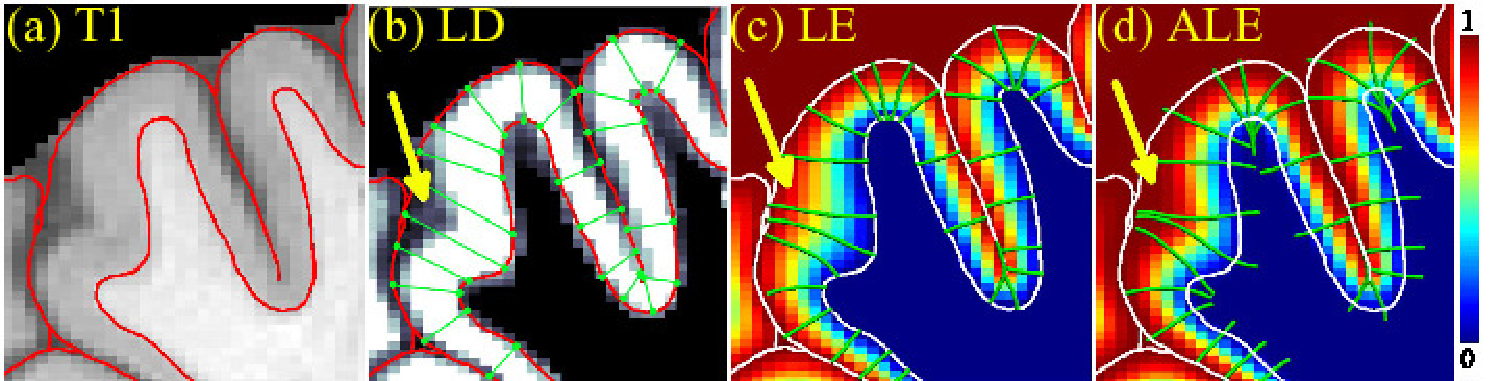
\includegraphics[width=1\textwidth]{fig/threemethods} 
\par\end{centering}
\caption{(a) Inner and pial surface boundaries overlaid on T1-weighted image;
(b) cortical thickness computation based on linked distance overlaid on the gray matter fraction image (LD);
(c) the solutions of the Isotropic Laplace Equation (LE) and (d) the
proposed ALE method are shown as a color coded temperature distribution
with green lines depicting the streamlines. The yellow arrow depicts
an example region where the three methods differ significantly. \label{fig:(a)-Inner-and}}
\end{figure}
Fig. 1 illustrates the color coded temperature distribution solution to the ALE in a 2D section of cortex
in comparison to the solution of the isotropic LE and the LD method within $\Omega$.
We also show corresponding streamlines for the ALE using partial tissue
fractions relative to those for the isotropic case. Note that the green streamlines in Fig 1 (d) extend into the white matter due to the non-zero gray matter fraction in this region. Integrals of $\phi_{\infty}(v)$
over these streamlines from inner to pial surface can be used to compute
thickness \cite{evans_partial_2009}. We propose an alternative
simple analytic expression by defining the cortical thickness $T(v)$
at each point on the mid-cortical surface as: 
\begin{align}
T(v) & =f(v)\frac{1}{\left\Vert \nabla\phi_{\infty}(v)\right\Vert },\,\text{where}\,(v)\in\partial\Omega{}_{mid}.\label{eq:Thickness_expression}
\end{align}
Here the mid-cortical surface $(\partial\Omega)_{mid}$ is defined
as the level set: $(\partial\Omega)_{mid}=\left\{ v\in\mbox{\ensuremath{\Omega}}|\phi_{\infty}(v)=\frac{1}{2}\right\} .$
The analytic expression in Eq. \ref{eq:Thickness_expression} is shown
in Section \ref{subsec:Analytic-Solution-to} to be equivalent to
the path integral for the 1-dimensional solution to the ALE, not only
at $(\partial\Omega)_{mid}$ but at all points with non-zero gray
matter fraction. An intuitive explanation of why this approximation
works is as follows. We impose boundary conditions of temperatures
0 and 1 on the inner and pial surfaces, respectively. So for homogeneous
gray matter the temperature gradient between them, $\left\Vert \nabla\phi_{\infty}(v)\right\Vert $,
will be inversely proportion to thickness. Consequently, calculation
of the reciprocal of the gradient at the midcortical surface should
produce a good estimate of thickness. For the anisotropic case, we
account for the increased flux in partial volume voxels that may lie
on the mid-cortical surface by scaling by the gray matter fraction
$f(v)$.

\subsection{Analysis using a 1D Model \label{subsec:Analytic-Solution-to}}

To illustrate how ALE works, we use a 1D model. %and show that the ALE method is robust to blurring with kernels that integrate
%to unity (e.g., Gaussian smoothing). 
In this model we assume pure white matter is the region from
$x=$ -$\infty$ to $-L$, the cortex (containing gray matter) from
$x=-L$ to $L$, and pure CSF from $x=L$ to $\infty.$ We assume
an arbitrary gray matter fraction distribution $f(x)$ on $(-L,L)$.
We then blur this distribution with a kernel $g(x)$ with the property
$\intop_{-\infty}^{\infty}g(x)=1$. Following Eq. \ref{eq:Thickness_expression},
we obtain the thickness 
\begin{equation}
T=h(x)\left(\frac{d\phi_{\infty}(x)}{dx}\right)^{-1}\text{at}\ x:\phi_{\infty}(x)=0.5.\label{eq:thick_1D}
\end{equation}
Here $h(x)=f(x)$ for the unblurred case and $h(x)=f(x)\circledast g(x)$
for the blurred case, where $\circledast$ indicates convolution.

The 1D anisotropic heat equation is $\frac{\partial\phi(x,t)}{\partial t}=\frac{\partial}{\partial x}\left(\frac{1}{f(x)}\frac{\partial\phi(x,t)}{\partial x}\right)\,$
for the unblurred case, with boundary conditions $\phi(-L,t)$ = 0
and $\phi(L$,t) = 1. Solving for $\phi_{\infty}(x)$ gives $\phi_{\infty}(x)=\nicefrac{\intop\limits _{-L}^{x}f(y)dy}{\intop\limits _{-L}^{L}f(y)dy}$.
Substituting this into Eq. \ref{eq:thick_1D} gives the correct value
$T=\intop_{-L}^{L}f(y)dy\,.$ It is somewhat surprising that the thickness
value computed in this manner does not depend on the point $x$ at
which it is computed in Eq. \ref{eq:thick_1D}, although for consistency
of definition, we always compute it at the mid point between inner
and outer boundary.

Now if we blur the gray matter fraction with a unit-integral kernel,
solve the heat equation in steady state, and substitute in Eq. \ref{eq:thick_1D},
the resulting solution is $T=\intop_{-\infty}^{\infty}\intop_{-\infty}^{\infty}f(x)g(y-x)\,dx\,dy=\intop_{-\infty}^{\infty}f(x)\left(\int_{-\infty}^{\infty}g(y-x)\,dy\right)\,dx=\intop_{-L}^{L}f(x)\,dx\ \int_{-\infty}^{\infty}g(y)\,dy=\intop_{-L}^{L}f(x)\,dx.$
In other words, the thickness calculations using ALE is unaffected
by blurring with a sufficiently narrow kernel with unit integral,
provided the blurred gray matter fraction of the cortex lies within
the bounds defined by the inner and pial surfaces. It should be noted
that in the 3D case, blurring of the image will lead to some smoothing
of the computed thickness values along the surface, but this should
not add bias to the thickness values.

\section{Applications and Results}

\subsection{Average Cortical Thickness Study \label{subsec:methods avg_cortical_thickness1}}

We analyzed 3D structural brain MRI scans of 198 normal right handed
subjects (76 male, 122 female, age range: 18-26 years) from the 1000
Functional Connectomes Project \url{http://fcon_1000.projects.nitrc.org}.
Images were acquired using MPRAGE on a SIEMENS TRIO 3T scanner: TR
= 2530 ms, TE = 3.39 ms, slice thickness = 1.33 mm, flip angle = 7\textdegree ,
inversion time = 1100 ms, FOV = 256 mm \texttimes{} 256 mm, in-plane
resolution = 256 \texttimes{} 192, 128 slices. We used the BrainSuite
software (\url{http://brainsuite.org}) \cite{shattuck_brainsuite:_2002}
to define the partial volume fractions, as well as for extracting
inner and pial cortical surfaces. All cortical surfaces were aligned
to a common atlas space using BrainSuite in order to compute population
based averages. Cortical thicknesses were computed as described in
Section \ref{sec:ALEmethod} where we used a finite difference method
to solve the anisotropic Laplace equation. 
\begin{figure}
\begin{centering}
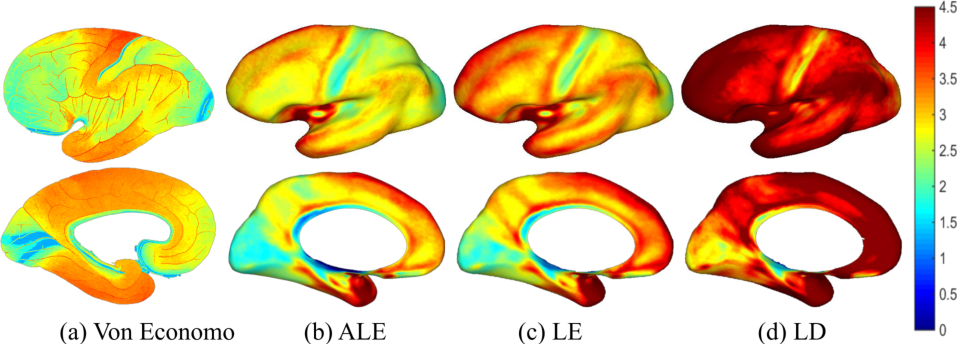
\includegraphics[width=1\textwidth]{fig/avg_thickness_cont_miccai} 
\par\end{centering}
\caption{(a) Histology based thickness map from Von Economo \cite{von_economo_cytoarchitectonics_1925};
(b)-(d)Average cortical thickness maps of left hemisphere. Lateral
(upper) and medial (lower) views from N=198 adult subjects computed
using: (b) Anisotropic Laplace Equation (ALE), (c) Isotropic Laplace
Equation (LE), and (d) Linked Distance (LD). \label{Figure: continuous maps of average cortical thickness} }
\end{figure}

We processed each of the 198 subject images using three methods: LD,
LE and ALE, and mapped these to the atlas to compute the point-wise
average cortical thickness on the surface. A surface based Laplace-Beltrami
isotropic smoothing \cite{joshi_parameterization-based_2009} of \textasciitilde{}10
mm fwhm was applied to the thickness estimates in the original subject
surface to compensate for discretization and small misregistration
errors. We used a robust mean estimate in which outliers (the 5\%
most extreme values) were first removed for each vertex on the surface.
The maps of average cortical thickness estimated are shown in Fig.
\ref{Figure: continuous maps of average cortical thickness}(b)-(d).
For comparison we include in Fig. \ref{Figure: continuous maps of average cortical thickness}(a)
a pseudo-colored version of Von Economo's map of cortical thickness
from \cite{von_economo_cytoarchitectonics_1925} which is based on
histological measurements.
\begin{figure}[th]
\centering{}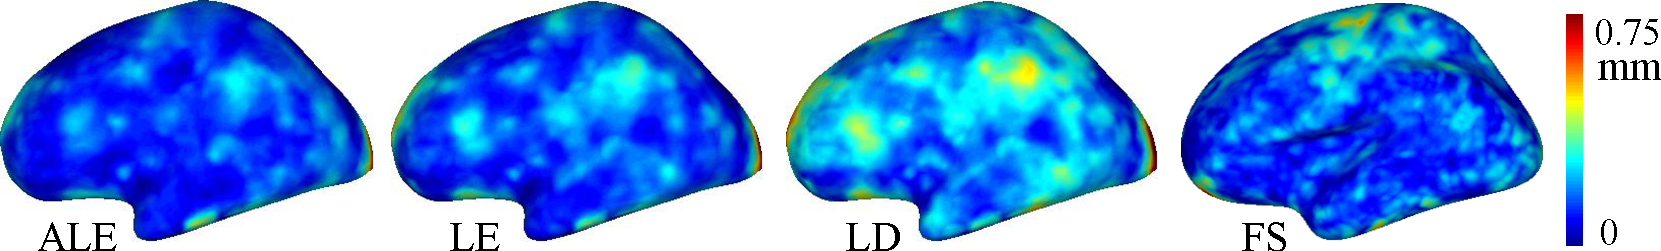
\includegraphics[width=1\textwidth]{fig/jessica1_cropped_miccai_v2}\caption{Effect of scanner differences on cortical thickness estimates for
four methods: absolute thickness difference between estimates from
the Siemens Trio 3T and Siemens Avanto 1.5T scanners, averaged over
5 subjects. ALE = Anisotropic Laplace Equation, LE = Laplace Equation,
LD = Linked Distance, FS = FreeSurfer. \label{fig: 3 T vs 1p5 T scanner thickness difference} }
\end{figure}
The patterns of thickness variation across the cortex are similar
for all three methods, however the range of values is quite different.
The cortical thickness estimates found using ALE were more consistent
with the Von Economo estimates in the parietal, occipital and temporal
lobes, while they were different in the frontal lobe. It should be
noted that the demographics of the subjects used in the histological
study was different than the imaged population. Von Economo and Koskinas
used brains of mentally healthy Caucasian subjects, 30\textendash 40
years of age \cite{triarhou_economo-koskinas_2007} whereas the population
in the data we used had an age range of 18-26 and were scanned in
Beijing. This difference in the demographics, and especially the younger
population in our study, may account for some of the increased thickness
in the frontal lobe \cite{gogtay_dynamic_2004}. LE shows higher thickness
than the Von Economo estimates everywhere on the cortex and LD showed
even higher values. A similar comparison using FreeSurfer based thickness
computation method was presented in \cite{scholtens_linking_2015}
where it was shown that FreeSurfer also tended to overestimate the
cortical thickness, although the pattern of cortical thickness was
similar.


%\subsection{Effect of Resolution Differences\label{subsec:methods Effect-of-Resolution}}

%The purpose of this study was to analyze the effect of changes
%in scan resolution on thickness estimates. This was done by computing
%the cortical thickness from both a high resolution and a downsampled
%image of a single subject. A high-resolution (0.5 mm X 0.5 mm X 0.8 mm)
%whole brain MRI was acquired using 3D MPRAGE scan of a right-handed
%dult woman in her mid-thirties, acquired at USC's Dornsife Cognitive
%euroscience Imaging Center on a 3T Siemens MAGNETOM Tim Trio scanner.
%\begin{figure}
%\begin{centering}
%\includegraphics[width=1\textwidth]{fig/hires_lowres_miccai} 
%par\end{centering}
%\caption{Effect of resolution on cortical thickness estimations for three methods:
%absolute value of differences in thickness estimated for high and
%low resolution images. \label{fig:low_high_res}}
%end{figure}
%A lower resolution version of this image was obtained by downsampling
%to a resolution of 1 mm x 1 mm x 1 mm by truncating raw k-space data.
%he BrainSuite surface extraction sequence was used to find the inner
%nd pial surfaces for both images. The three methods were then
%applied to estimate cortical thickness from both data sets. The thickness
%estimates were mapped to a common atlas for comparison using BrainSuite. A surface based Laplace-Beltrami isotropic
%smoothing \cite{joshi_parameterization-based_2009} of \textasciitilde{}10
%mm fwhm was applied to the thickness estimates in the original subject
%urface to compensate for discretization and mis-registration errors.
%The cortical maps of the thickness differences are shown in Fig. \ref{fig:low_high_res}. In these difference maps the LD methods shows by far the largest difference
%followed by LE whereas ALE shows the least difference, reflecting the design of ALE to be robust to resolution differences. The areas of largest difference in ALE are in the insula (also present in LE and LD) which possibly arises from the inclusion of the claustrum in the partial volume voxels associated with insula gray matter. 


\subsection{Test-Retest Reliability Study for Multiple Scanners}
\label{subsec:methods-multiple scanner single sessions} 

\begin{wrapfigure}{r}{0.50\textwidth}%
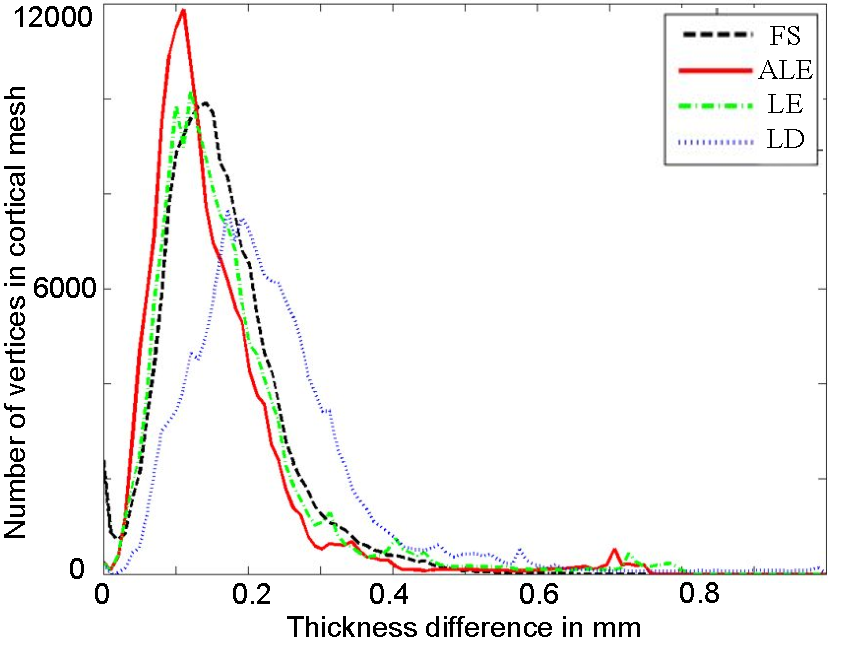
\includegraphics[width=0.50\textwidth]{fig/Hist_Jessica}
\vspace{-20pt}
\caption{Histogram of the average absolute differences between thickness measures
for ALE, LE, LD and FS for 1.5T Siemens Avanto and 3T Siemens Trio
scanners. \label{fig: 3T vs 1p5 histogram} }
\vspace{-20pt}
\end{wrapfigure}%
The purpose of this study was to analyze the effects of scanner differences
on cortical thickness measurements in the same subject. The data for
this study consisted of 5 normal subjects scanned on two different
scanners. All the scans were acquired within three days at the University
of Iowa. The first scan was acquired using a Siemens Trio 3T scanner: slice
thickness 1 mm, TR 2530, TE 3.99 ms, inversion time 1100 ms, in-plane
resolution 1 $\textrm{mm}^{2}$ and flip angle $10^{\circ}$. The
second scan was acquired using a Siemens Avanto 1.5T scanner: slice
thickness 1.5 mm, TR 26 ms, TE 7 ms, in-plane resolution 1.066 $\text{mm}^{2}$
and flip angle $30^{\circ}$. The BrainSuite surface extraction pipeline
was executed for all scans. Thickness estimates were computed using
the three methods and coregistered to the atlas brain using BrainSuite.
In addition, we also executed the FreeSurfer pipeline (Version 5.3.0)
on these subjects. Laplace-Beltrami surface based smoothing \textasciitilde{}10
mm fwhm was applied and thickness differences were computed. The absolute
value of thickness difference corresponding to 3T and 1.5T Siemens
scanners, averaged over the five subjects was computed for all four
methods as shown in Fig. \ref{fig: 3 T vs 1p5 T scanner thickness difference}.
We also show histograms of these differences in Fig. \ref{fig: 3T vs 1p5 histogram}.
As with the simulation study, the ALE method shows the smallest absolute
difference (mean 0.1575mm, sd 0.1034mm) between the 3T vs 1.5T scanners
relative to LE (mean 0.1786mm, sd 0.1163mm) and LD (mean 0.2480mm, sd
0.1520mm), and FreeSurfer (mean 0.1679mm, sd 0.0821mm).


\section{Discussion and Conclusion}

Studies of cortical thickness usually compare differences in thickness
in homologous areas between two groups, or changes in thickness over
time during maturation, aging or disease progression. For this reason,
consistency and robustness of thickness estimates is possibly as important
as absolute accuracy. For this reason, we examined not only the average
cortical thickness over a relatively larger population, but also the
consistency of thickness estimates among subjects scanned in two different
scanners. The study of 198 subjects produced average thicknesses with
the ALE method that are more in line with those reported in the literature
using histological studies than the alternative LE and LD methods.
Differences in the frontal lobe using ALE compared to the values in
the Von Economo atlas are consistent with age differences in the two
different populations studied and reported changes in thickness in
early adulthood in frontal cortex \cite{gogtay_dynamic_2004}.

The consistency study in Figs. \ref{fig: 3 T vs 1p5 T scanner thickness difference}
and \ref{fig: 3T vs 1p5 histogram} shows that there is a consistent
bias in all methods in the thickness estimates computed from images
from the 3T scanner versus those from the 1.5T. However, the histograms
of these differences confirm the reduced sensitivity to differences
 in resolution of the ALE method relative to FS, LE and LD. % This follows
% from the explicit use of partial volume fractions in the thickness
% calculation and the robustness of thickness measures, which we illustrated
% for the 1D case, to blurring of the image.
% Computation cost is typically not a major consideration when analyzing
% brain data, but we note that improved performance is achieved with
% higher computation cost. The poorest performing methods computes linked
% distances in approximately 5 seconds on a typical laptop. The isotropic
% Laplace equation method takes 10 minutes while the anisotropic Laplace
% method requires approximately 15 minutes per subject. Computing thickness
% with ALE using the approximation in Eq. \ref{eq:Thickness_expression}
% rather than integrating along streamlines significantly reduces the
% total cost.

In summary, results presented here indicate that ALE is capable of
producing cortical thickness estimates that are largely consistent
with those reported from histological measurements, and that these
estimates are less sensitive to the effects of imaging in a different
scanner for the limited range of conditions over which we have so
far studied this method. Further evaluation is required, and as with
all thickness estimation methods, though inter-scanner differences
may be reduced, our results indicate that it is important that scanner-dependent
effects be factored into any subsequent analysis.

 \bibliographystyle{splncs04}
\bibliography{Mybib}

\end{document}
